Για τη δεύτερη άσκηση συνθέτουμε μια αριθμομηχανή η οποία αξιοποιεί την $alu$ της
προηγούμενης άσκησης. Δημιουργούμε δύο αρχεία:
\begin{itemize}
    \item \textbf{$calc_enc\.v:$} Υλοποιεί με $structural verilog$ το σήμα $alu_op$ βάσει 
    της κατάστασης των τριών κουμπιών ($btnr$, $btnc$, $btnl$), 
    \item \textbf{$calc\.v:$} Συγκεντρώνει τη λειτουργικότητα των $alu$, $calc_enc$ και 
    επιπρόσθετα ενημερώνει τον συσσωρευτή βάσει της κατάστασης των κουμπιών $btnu$ και $btnd$.
    Επίσης φροντίζει να αντικατοπτρίζεται ο συσσωρευτής στο $LED$ και δημιουργεί με επέκταση 
    προσήμου δύο $32-bit$ εκδοχές του συσσωρευτή και του διακόπτη για να τις προωθήσει στην
    $alu$ η οποία δέχεται $32-bit$ εισόδους.
\end{itemize}

Κυματομορφές προσομοίωσης:
\begin{figure}[H]
    \centering
    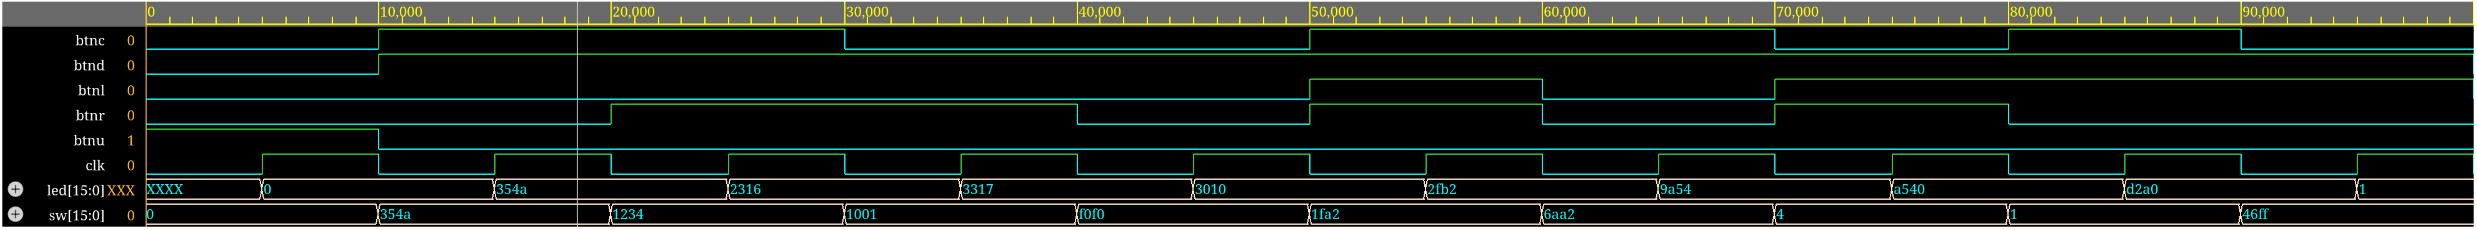
\includegraphics[width=0.5\textwidth]{media/exercise2_waveforms.png}
\end{figure}